% =====================================================================
%  Deterministic vs SFLT-stochastic field comparison (strong noise),
%  Williamson 6 and Williamson 5. Requires \usepackage{graphicx}.
%  Each PNG is a 2-panel lon-lat map: deterministic (left) | SFLT (right),
%  matched colour scale.
% =====================================================================

% ---------- Williamson 6 ----------
\begin{figure}[htbp]
  \centering
  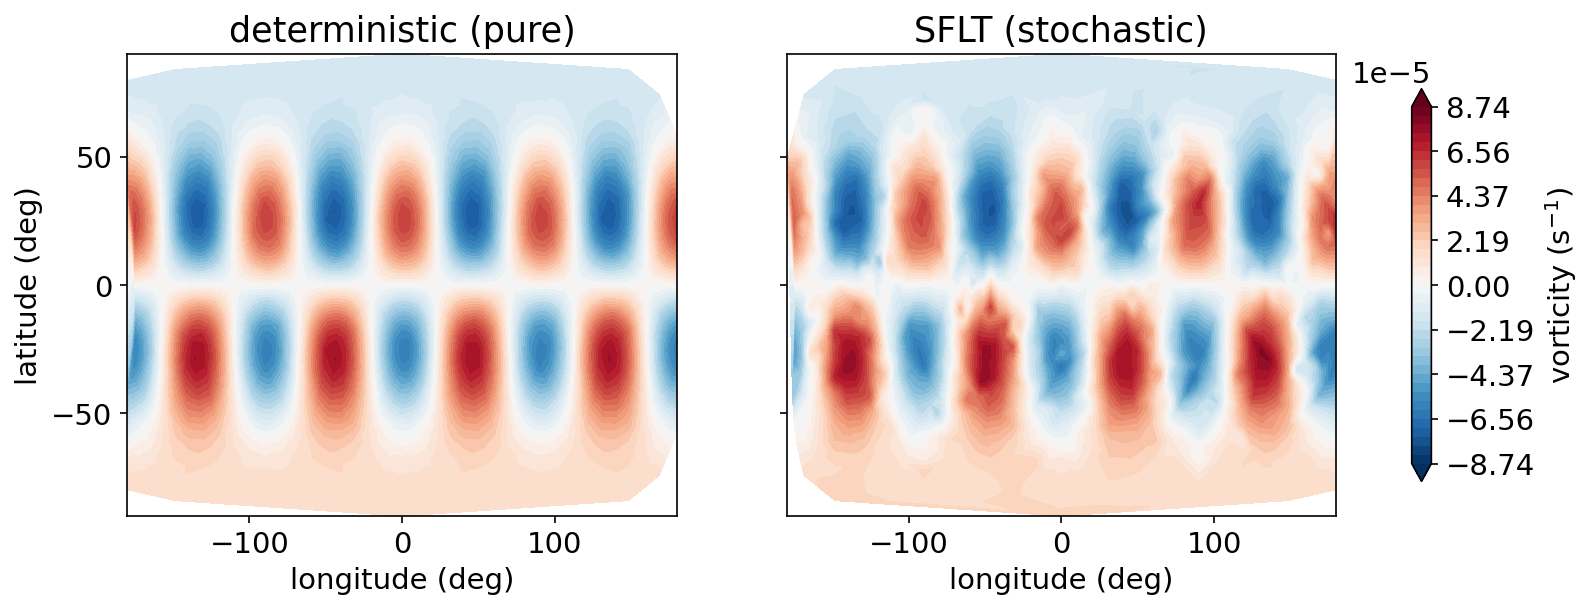
\includegraphics[width=\textwidth]{w6_compare_vorticity.png}
  \caption{Relative vorticity for Williamson test case~6 at $t = 2$ days,
    refinement level~5: deterministic run (left) versus SFLT stochastic run at
    strong noise amplitude ($u_{\mathrm{noise}}/u \approx 0.5$, right), on a
    common colour scale. The stochastic transport noise injects small-scale
    vorticity filaments that are absent from the smooth deterministic
    Rossby--Haurwitz pattern, while the large-scale wavenumber-4 structure is
    retained. The amplitude is deliberately strong here for visualisation; the
    same divergence-free, energy-conserving noise underlies the conservation
    results (Figs.~\ref{fig:sflt-amp-sweep}, \ref{fig:sflt-ensemble-energy}).}
  \label{fig:w6-compare-vort}
\end{figure}

\begin{figure}[htbp]
  \centering
  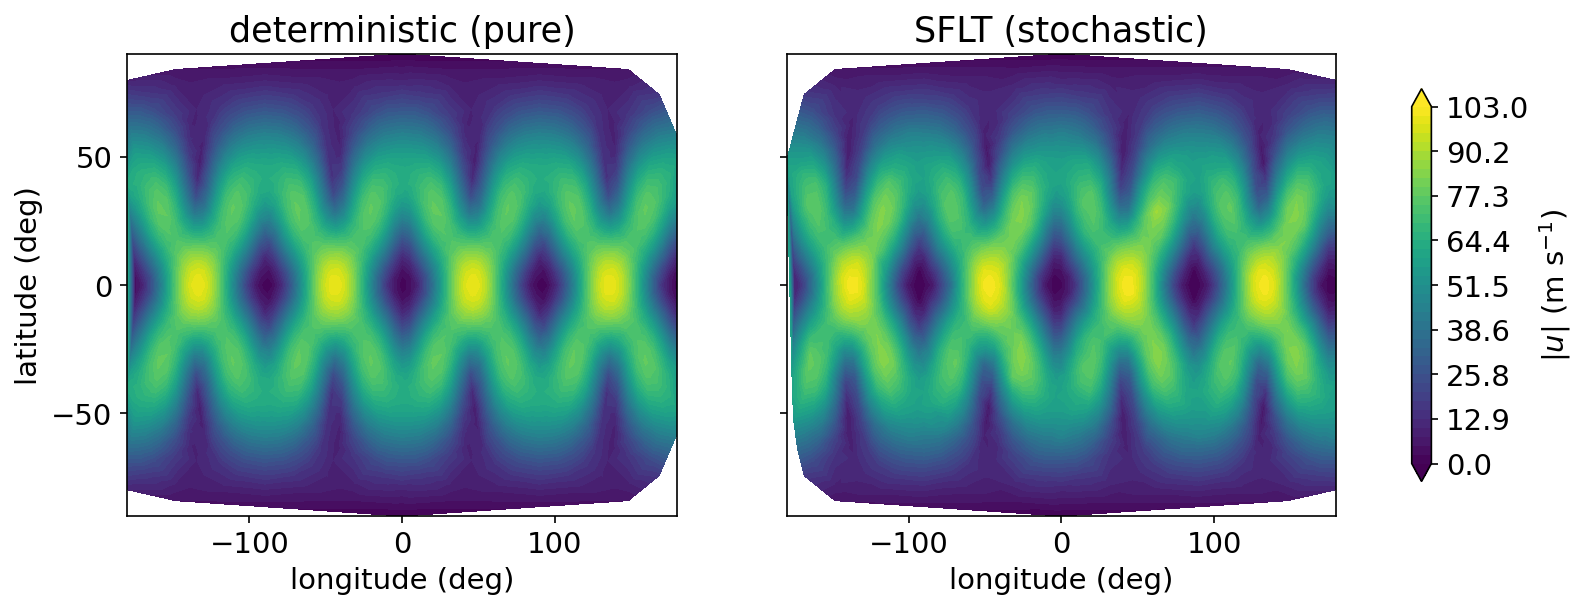
\includegraphics[width=\textwidth]{w6_compare_velocity.png}
  \caption{Velocity magnitude $|u|$ for Williamson test case~6 at $t = 2$ days,
    deterministic (left) versus SFLT at $u_{\mathrm{noise}}/u \approx 0.5$
    (right), common colour scale. At this strong amplitude the noise is visible
    even in the speed field as a small-scale texture superimposed on the
    large-scale flow.}
  \label{fig:w6-compare-vel}
\end{figure}

% ---------- Williamson 5 ----------
\begin{figure}[htbp]
  \centering
  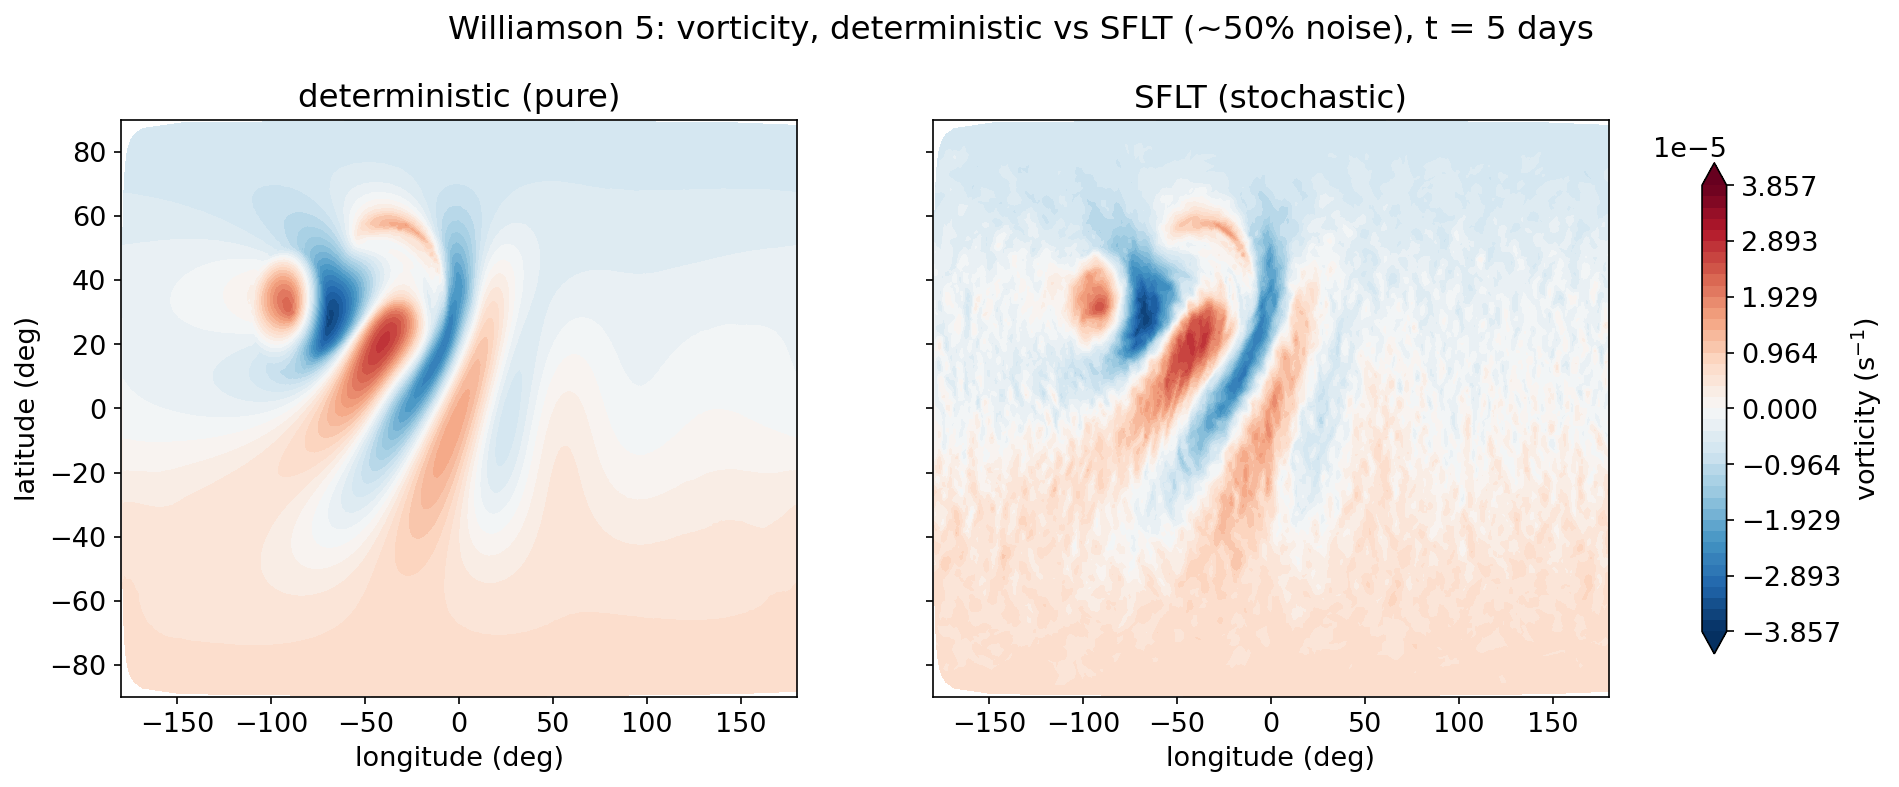
\includegraphics[width=\textwidth]{w5_compare_vorticity.png}
  \caption{Relative vorticity for Williamson test case~5 (flow over a mountain) at
    $t = 5$ days, refinement level~5: deterministic run (left) versus SFLT
    stochastic run at strong noise amplitude ($u_{\mathrm{noise}}/u \approx 0.5$,
    right), common colour scale. The noise adds small-scale eddies superimposed on
    the mountain-forced lee-wave and Rossby-wave-train vorticity of the
    deterministic solution.}
  \label{fig:w5-compare-vort}
\end{figure}

\begin{figure}[htbp]
  \centering
  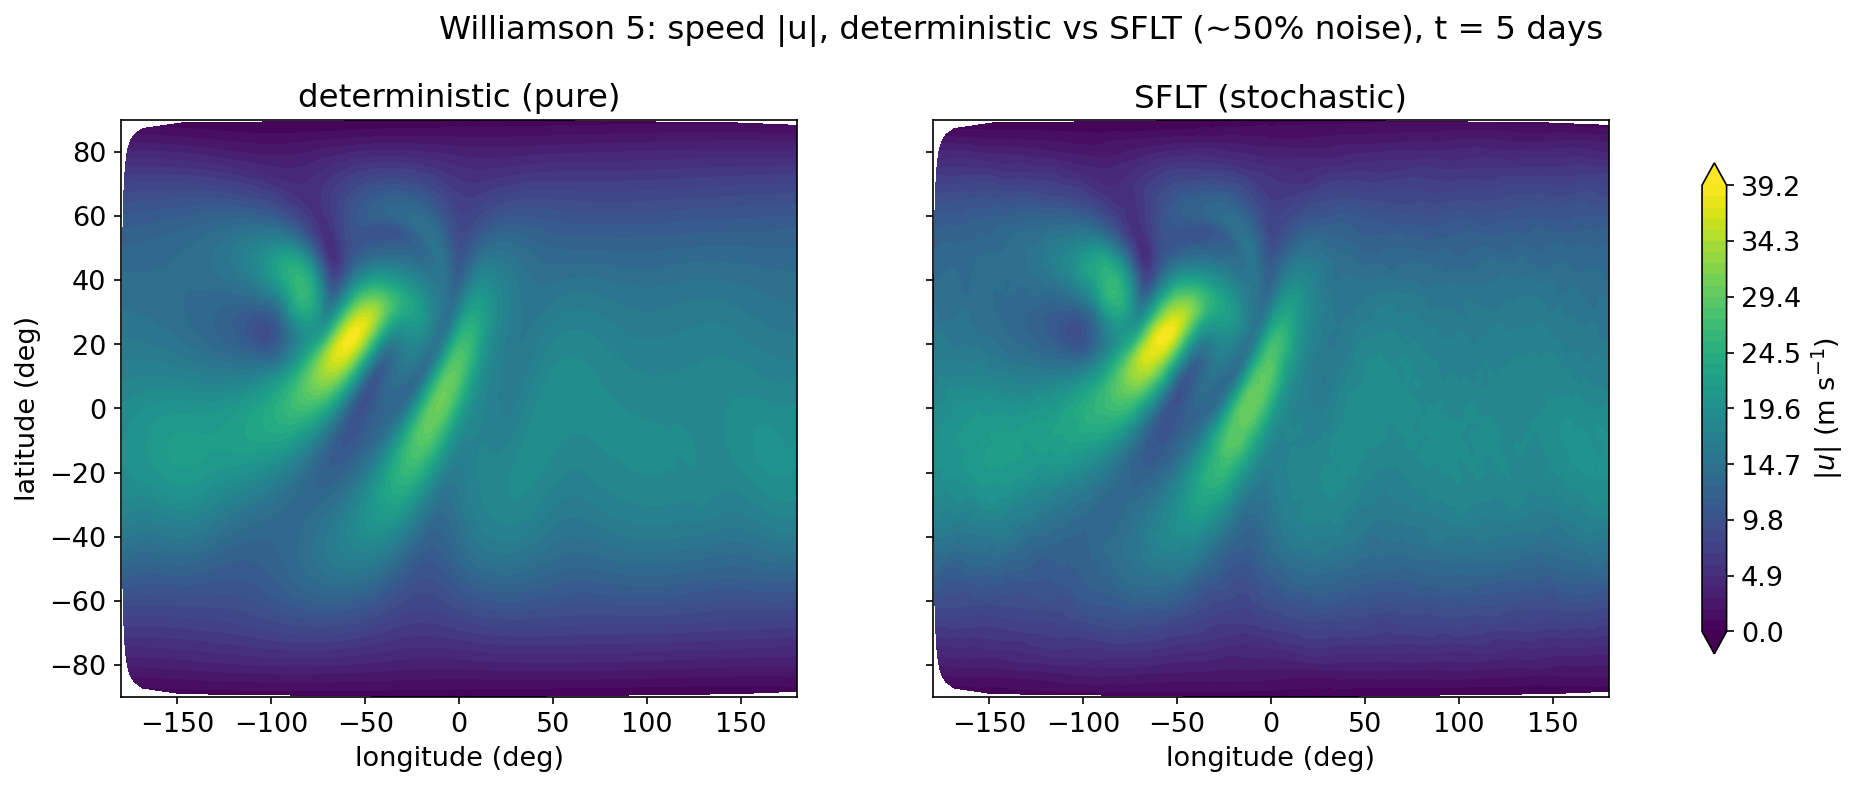
\includegraphics[width=\textwidth]{w5_compare_velocity.png}
  \caption{Velocity magnitude $|u|$ for Williamson test case~5 at $t = 5$ days,
    deterministic (left) versus SFLT at $u_{\mathrm{noise}}/u \approx 0.5$
    (right), common colour scale.}
  \label{fig:w5-compare-vel}
\end{figure}
